% Note: this need to be compiled twice! 
\documentclass[11pt,twocolumn,landscape,a4paper,notitlepage]{article}

% Packages
\usepackage{calc}			% for length arithmetic.
\usepackage[twocolumn, top=1.0cm, bottom=1.0cm, left=1.0cm, right=1.0cm, voffset=0cm, hoffset=0cm, headsep=0.2cm, headheight=13.6pt, footskip=\headsep + \headheight, columnsep=1.25cm]{geometry}
\usepackage{babel}
\usepackage{listings} 				% for code snippets.
\usepackage{fancyhdr}				% for headers and footers.
\usepackage{etoolbox}				% for the \maketitle hack.
\usepackage{array}					% for table column specifications.
\usepackage{graphicx}				% for table resize.
\usepackage{booktabs}				% for tables.
\usepackage{xtab}					% for multiple pages tables.
\usepackage[hidelinks]{hyperref}	% for click-able toc
\usepackage{amsmath}
\usepackage{graphicx}
\usepackage{ragged2e}
\usepackage{xcolor}

\lstnewenvironment{code}
    {%\lstset{	numbers=none, frame=lines, basicstyle=\small\ttfamily, }%
    \csname lst@SetFirstLabel\endcsname}
    {\csname lst@SaveFirstLabel\endcsname}
% We create some new table columns types.
\newcolumntype{L}[1]{>{\raggedright\let\newline\\\arraybackslash\hspace{0pt}}m{#1-2\tabcolsep- 1.25\arrayrulewidth}}
\newcolumntype{C}[1]{>{\centering\let\newline\\\arraybackslash\hspace{0pt}}m{#1-2\tabcolsep- 1.25\arrayrulewidth}}
\newcolumntype{R}[1]{>{\raggedleft\let\newline\\\arraybackslash\hspace{0pt}}m{#1-2\tabcolsep- 1.25\arrayrulewidth}}

% We make visible heder's and footer's ruler.
\renewcommand{\headrulewidth}{0.5pt}
\renewcommand{\footrulewidth}{0.5pt}
\renewcommand{\columnseprule}{0.5pt}

% To display the footer and header on the first page.
\fancypagestyle{plain}
{
	\fancyhf{}
	\rhead{I'm one with the code, the code is one with me}
	\lhead{UTN FRSF - Champ\'an en Lata}
	\rfoot{P\'agina \thepage}
}
\pagestyle{plain}

% and for the rest of the pages.
\fancyhf{}
\rhead{\leftmark}
\lhead{UTN FRSF - Champ\'an en Lata}
\rfoot{P\'agina \thepage}

% We use Courier font to make bold keywords possible.
\renewcommand{\ttdefault}{pcr}

\usepackage{xcolor}
\definecolor{commentgreen}{RGB}{2,112,10}

% Listing code style
\lstdefinestyle{codestyle}{
	basicstyle=\scriptsize\ttfamily,
    keywordstyle=\bfseries,
    emph={int,char,double,float,unsigned,void,bool},
    emphstyle=\bfseries,
    breakatwhitespace=false,
    breaklines=true,
    captionpos=b,
    keepspaces=false,
    numbers=left,
    numberstyle=\tiny\ttfamily,
    numbersep=5pt,
    frame=single,
    framesep=3pt,
    showspaces=false,
    showstringspaces=false,
    showtabs=false,
    tabsize=2,
    commentstyle=\color{commentgreen}, % comment color
    keywordstyle=\color{blue}, % keyword color
    stringstyle=\color{red} % string color
}
\lstset{style=codestyle}

% To dislpay the title on one column 
\makeatletter
% Remove the brackets so LaTeX sees \twocolumn\@maketitle
\patchcmd{\maketitle}{[\@maketitle]}{\@maketitle}{}{}
% Remove the vertical shift from the title 
\patchcmd{\@maketitle}{\null\vskip2em\begin{center}}{\vspace*{0pt}\nointerlineskip\begingroup\centering}{}{}
% In the final part we must remove \end{center}
\patchcmd{\@maketitle}{\end{center}\par}{\par\endgroup}{}{}
\makeatother


% Information
\author{UTN FRSF - Champ\'an en Lata}
\title{El Mufoso}
\date{2025}


\begin{document}
\maketitle
\centering{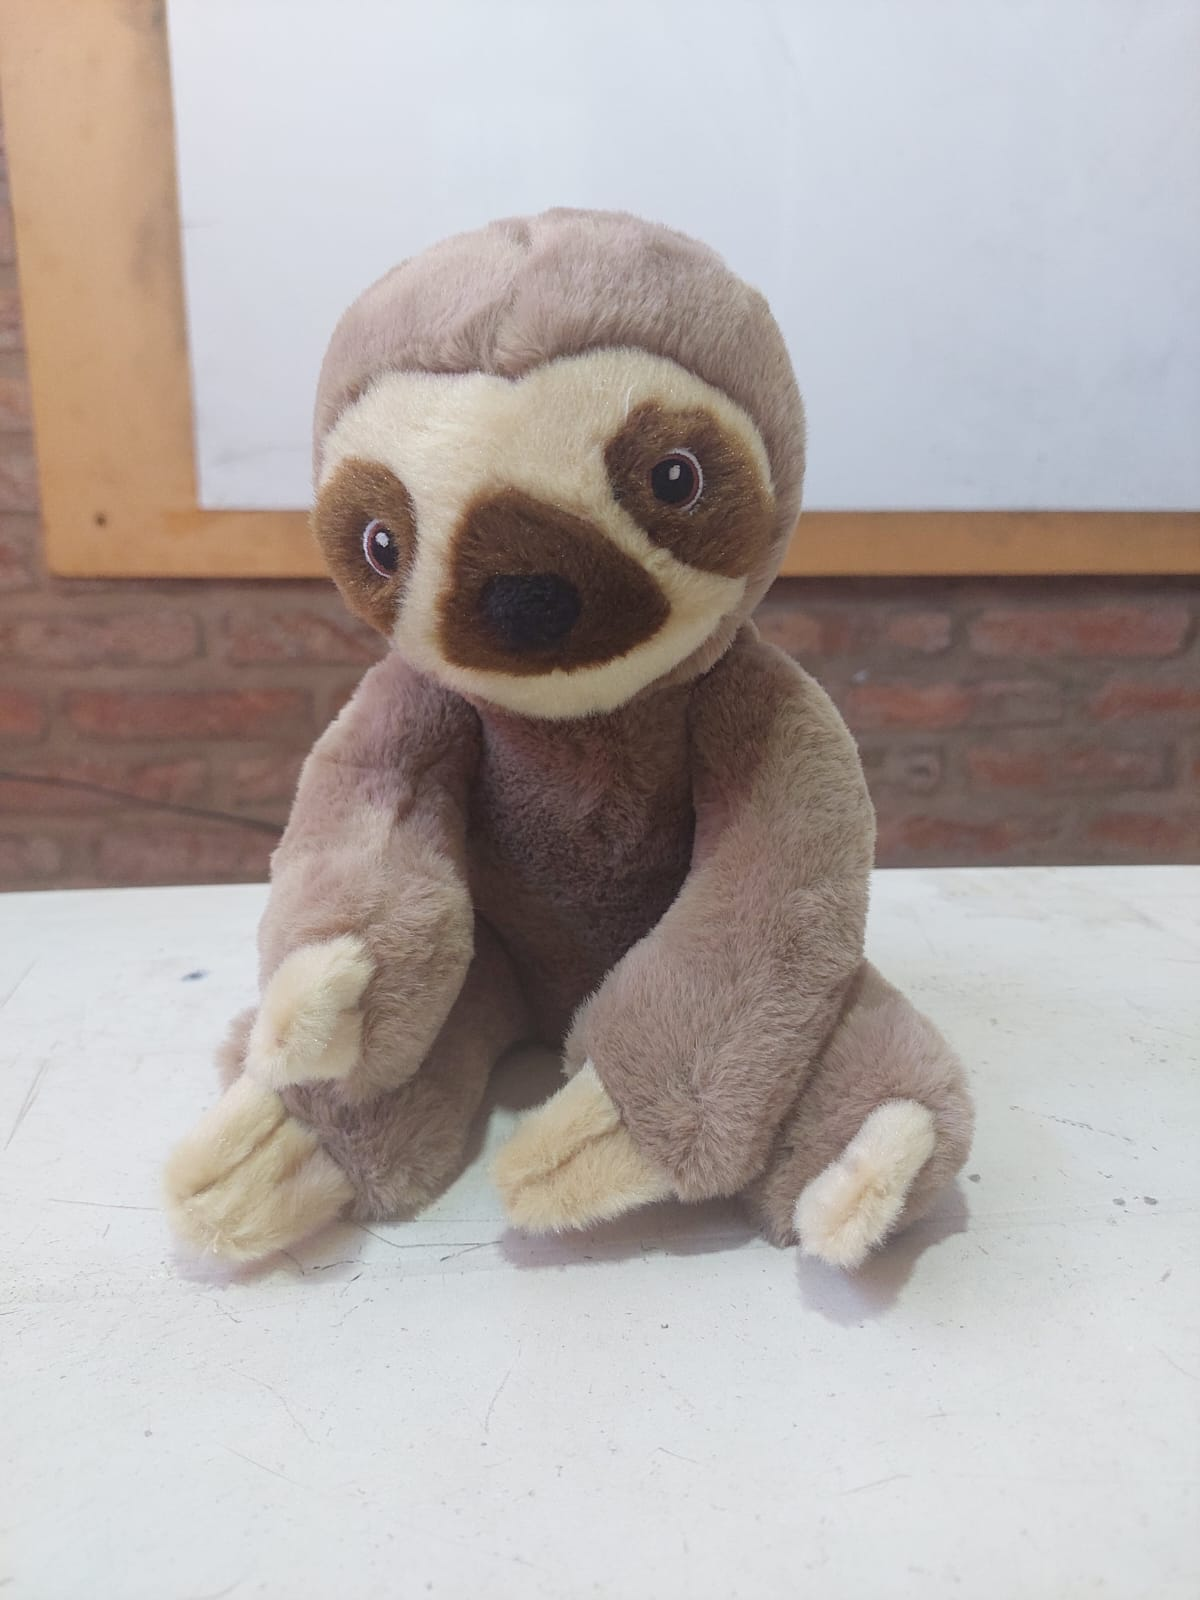
\includegraphics[width=7cm]{elnuevooso.jpeg}}
\tableofcontents
\newpage

% Here we include each section of this notebook from external files.
\input{./secciones/template/template.tex}
\newpage
\section{Math}

\subsection{Identidades}
{
$\sum_{i=0}^n\binom{n}{i}=2^n$

$\sum_{i=0}^n i\binom{n}{i}=n*2^{n-1}$

$\sum_{i=m}^n i = \frac{n(n+1)}{2} - \frac{m(m-1)}{2} = \frac{(n+1-m)(n+m)}{2}$

$\sum_{i=0}^n i = \sum_{i=1}^n i = \frac{n(n+1)}{2}$

$\sum_{i=0}^n i^2 = \frac{n(n+1)(2n+1)}{6} = \frac{n^3}{3} + \frac{n^2}{2} + \frac{n}{6}$

$\sum_{i=0}^n i(i-1) = \frac{8}{6}(\frac{n}{2})(\frac{n}{2}+1)(n+1)$ (doubles) $\rightarrow$ Sino ver caso impar y par

$\sum_{i=0}^n i^3 = \left(\frac{n(n+1)}{2}\right)^2 = \frac{n^4}{4} + \frac{n^3}{2} + \frac{n^2}{4} = \left[\sum_{i=1}^n i\right]^2$

$\sum_{i=0}^n i^4 = \frac{n(n+1)(2n+1)(3n^2+3n-1)}{30} = \frac{n^5}{5} + \frac{n^4}{2} + \frac{n^3}{3} - \frac{n}{30}$

$\sum_{i=0}^n i^p = \frac{(n+1)^{p+1}}{p+1} + \sum_{k=1}^p\frac{B_k}{p-k+1}{p\choose k}(n+1)^{p-k+1}$

$r=e-v+k+1$

Teorema de Pick: (Area, puntos interiores y puntos en el borde)

$A=I+\frac{B}{2}-1$


}%
\subsection{Ec. Caracteristica}
$a_0T(n)+a_1T(n-1)+...+a_kT(n-k)=0$

$p(x)=a_0 x^k + a_1 x^{k-1} + ... + a_k$

Sean $r_1,r_2,...,r_q$ las ra\'ices distintas, de mult. $m_1, m_2, ..., m_q$

$T(n)=\sum_{i=1}^q{\sum_{j=0}^{m_i - 1}c_{ij} n^j r_i^n}$

Las constantes $c_{ij}$ se determinan por los casos base.

\newpage
\subsection{Modular operations}
\lstinputlisting[language=C++]{secciones/math/modular_operations.cpp}
\subsection{Chinese reminder theorem, extended euclid and diophantine equations}
$$y=\sum_{j=1}^n (x_j*(\prod_{i=1, i\neq j}^n m_i)_{m_j}^{-1}*\prod_{i=1, i\neq j}^n m_i)$$
\newpage
\lstinputlisting[language=C++]{secciones/math/crt_euclid.cpp}
\subsection{Modular inverse}
\lstinputlisting[language=C++]{secciones/math/inversos.cpp}
\subsection{Combinatorics}
\lstinputlisting[language=C++]{secciones/math/combinatoria.cpp}

\subsection{Discrete Logarithm}
\lstinputlisting[language=C++]{secciones/math/discrete_log.cpp}

\newpage
\subsection{Fractions}
\lstinputlisting[language=C++]{secciones/math/fraction.cpp}

\subsection{Matrix exponentiation}
\lstinputlisting[language=C++]{secciones/math/matrix_exp.cpp}

\subsection{Primes, divisors and Phi}
\lstinputlisting[language=C++]{secciones/math/funciones_primos.cpp}
\newpage
\subsection{Phollard's Rho}
\lstinputlisting[language=C++]{secciones/math/phollard_rho.cpp}

\newpage
\subsection{Guass-Jordan}
\lstinputlisting[language=C++]{secciones/math/gauss_jordan.cpp}
\newpage
\subsection{Guass-Jordan modular}
\lstinputlisting[language=C++]{secciones/math/gauss_jordan_mod.cpp}
\newpage
\subsection{Guass-Jordan with bitset}
\lstinputlisting[language=C++]{secciones/math/gauss_jordan_bitset.cpp}

\subsection{Simpson}
\lstinputlisting[language=C++]{secciones/math/simpson.cpp}

\newpage
\subsection{Fast Fourier Transform (FFT)}
\lstinputlisting[language=C++]{secciones/math/fft.cpp}

\subsection{Karatsuba}
\lstinputlisting[language=C++]{secciones/math/karatsuba.cpp}

\newpage
\subsection{Simplex}
\lstinputlisting[language=C++]{secciones/math/simplex.cpp}

\subsection{Tablas y cotas (Primos, Divisores, Factoriales, etc)}
%\subsubsection{
\paragraph{Factoriales} \ \\
\begin{tabular}{l|l}
0! =	1             & 11! = 39.916.800  \\
1! =	1             & 12! =	479.001.600	($\in \mathtt{int}$)\\
2! =	2             & 13! =	6.227.020.800	\\
3! =	6             & 14! =	87.178.291.200	\\
4! =	24            & 15! =	1.307.674.368.000	\\
5! =	120   			  & 16! =	20.922.789.888.000	\\
6! =	720           & 17! =	355.687.428.096.000	\\
7! =	5.040	        & 18! =	6.402.373.705.728.000	\\
8! =	40.320	      & 19! =	121.645.100.408.832.000	\\
9! =	362.880       & 20! =	2.432.902.008.176.640.000	($\in \mathtt{tint}$) \\
10! =	3.628.800     & 21! =	51.090.942.171.709.400.000
\end{tabular}

%\subsubsection{
\paragraph{Primos} \ \\
2 3 5 7 11 13 17 19 23 29
31 37 41 43 47 53 59 61 67 71
73 79 83 89 97 101 103 107 109 113
127 131 137 139 149 151 157 163 167 173
179 181 191 193 197 199 211 223 227 229
233 239 241 251 257 263 269 271 277 281
283 293 307 311 313 317 331 337 347 349
353 359 367 373 379 383 389 397 401 409
419 421 431 433 439 443 449 457 461 463
467 479 487 491 499 503 509 521 523 541
547 557 563 569 571 577 587 593 599 601
607 613 617 619 631 641 643 647 653 659
661 673 677 683 691 701 709 719 727 733
739 743 751 757 761 769 773 787 797 809
811 821 823 827 829 839 853 857 859 863
877 881 883 887 907 911 919 929 937 941
947 953 967 971 977 983 991 997 1009 1013
1019 1021 1031 1033 1039 1049 1051 1061 1063 1069
1087 1091 1093 1097 1103 1109 1117 1123 1129 1151
1153 1163 1171 1181 1187 1193 1201 1213 1217 1223
1229 1231 1237 1249 1259 1277 1279 1283 1289 1291
1297 1301 1303 1307 1319 1321 1327 1361 1367 1373
1381 1399 1409 1423 1427 1429 1433 1439 1447 1451
1453 1459 1471 1481 1483 1487 1489 1493 1499 1511
1523 1531 1543 1549 1553 1559 1567 1571 1579 1583
1597 1601 1607 1609 1613 1619 1621 1627 1637 1657
1663 1667 1669 1693 1697 1699 1709 1721 1723 1733
1741 1747 1753 1759 1777 1783 1787 1789 1801 1811
1823 1831 1847 1861 1867 1871 1873 1877 1879 1889
1901 1907 1913 1931 1933 1949 1951 1973 1979 1987
1993 1997 1999 2003 2011 2017 2027 2029 2039 2053
2063 2069 2081
\newpage
\paragraph{Primos cercanos a $10^n$}\ \\
9941 9949 9967 9973 10007 10009 10037 10039 10061 10067 10069 10079\\
99961 99971 99989 99991 100003 100019 100043 100049 100057 100069\\
999959 999961 999979 999983 1000003 1000033 1000037 1000039\\
9999943 9999971 9999973 9999991 10000019 10000079 10000103 10000121\\
99999941 99999959 99999971 99999989 100000007 100000037 100000039 100000049\\
999999893 999999929 999999937 1000000007 1000000009 1000000021 1000000033
 
\paragraph{Cantidad de primos menores que $10^n$}\ \\
$\pi(10^1)$ = 4 ;
$\pi(10^2)$ = 25 ;
$\pi(10^3)$ = 168 ;
$\pi(10^4)$ = 1229 ;
$\pi(10^5)$ = 9592 \\
$\pi(10^6)$ = 78.498 ;
$\pi(10^7)$ = 664.579 ;
$\pi(10^8)$ = 5.761.455 ;
$\pi(10^9)$ = 50.847.534 \\
$\pi(10^{10})$ = 455.052,511 ;
$\pi(10^{11})$ = 4.118.054.813 ;
$\pi(10^{12})$ = 37.607.912.018% ;
%
% Fuente: http://primes.utm.edu/howmany.shtml#table
%
%

\subsection{N\'umeros Catalanes}
Utiles para problemas de Combinatoria


$Cat(n)=\frac{\binom{2n}{n}}{n+1} =\frac{(2n)!}{n!\,(n+1)!}$

Con $Cat(0)=1$.
\begin{flushleft}
Diferentes aplicaciones:

1. Contar la cantidad de diferentes arboles binarios con $n$ nodos que se pueden armar.

2. Contar las formas en que un pol\'igono convexo de $n+2$ lados puede ser triangulado.

3. Contar la cantidad de caminos monotonos a lo largo de los lados de una grilla $n*n$, que no cruzan la diagonal.

4. Contar el n\'umero de expresiones que contienen $n$ pares de par\'entesis correctamente colocados
\end{flushleft}

\subsubsection{Primeros 25 Catalanes}

\begin{flushleft}
1 1 2 5 14 42 132 429 1430 4862 16796 58786 208012 742900 2674440 
9694845 35357670 129644790 477638700 1767263190 6564120420
24466267020 91482563640 343059613650 1289904147324 4861946401452
\end{flushleft}

\input{./secciones/geometria/geometria.tex}
\input{./secciones/estructuras/estructuras.tex}
\input{./secciones/strings/strings.tex}
\input{./secciones/grafos/grafos.tex}
\input{./secciones/flow/flow.tex}
\input{./secciones/algoritmos/algoritmos.tex}
\newpage
\section{Juegos}
\subsection{Nim Game}
\begin{flushleft}
Juego en el que hay N pilas, con objetos. Cada jugador debe sacar al menos un objeto de una pila. GANA el jugador que saca el \'ultimo objeto.
\end{flushleft}
$P_0{\oplus}P_1{\oplus}...{\oplus}P_n = R$
\begin{flushleft}
Si $R{\neq}0$ gana el jugador 1.
\end{flushleft}

\subsubsection{Misere Game}
\begin{flushleft}
Es un juego con las mismas reglas que Nim, pero PIERDE el que saca el \'ultimo objeto. Entonces teniendo el resultado de la suma $R$, y 
si todas las pilas tienen 1 solo objeto $todos1{=}true$, podemos decir que el jugador2 GANA si:
\end{flushleft}
${(R{=}0){\&}{\neg}{todos1}{\parallel}(R{\neq}0 ){\&}{todos1}}$
\subsection{Ajedrez}
\subsubsection{Non-Attacking N Queen}
\begin{footnotesize}
	\textbf{Utiliza:} \texttt{<algorithm>}\\
	\textbf{Notas:} todo es $ O(!N \cdot N^{2})$.
\end{footnotesize}
\lstinputlisting[language=C++]{secciones/juegos/ajedrez_reinas.cpp}
\subsection{Green Hackenbush}
\lstinputlisting[language=C++]{secciones/juegos/green_hackenbush.cpp}

\input{./secciones/utils/utils.tex}


\end{document}
